\sloppy
\documentclass[14pt,a4paper,oneside]{extarticle}	% Размер основного шрифта и формата листа
\usepackage{xltxtra}						% Используется для вывода логотипа XeLaTeX
\usepackage{xunicode}						% Кодировка документа
\usepackage{polyglossia}					% Загружает пакет многоязыковой верстки
\newfontfamily\russianfont{Book Antiqua}
%\setmainfont{Liberation Serif}						% Основной шрифт текста
\setmainfont{Book Antiqua}
\setdefaultlanguage{russian}				% Основной язык текста
\setotherlanguage{english}					% Дополнительный язык текста
\linespread{1}							% Межстрочный интервал выбран полуторным
\usepackage[left=2.5cm,
right=1.5cm,vmargin=2.5cm]{geometry} % Отступы по краям листа
\bibliographystyle{ugost2008}

\usepackage{xcolor}
\usepackage{hyperref}
% Цвета для гиперссылок
\definecolor{linkcolor}{HTML}{359B08} % цвет ссылок
\definecolor{urlcolor}{HTML}{799B03} % цвет гиперссылок
\hypersetup{pdfstartview=FitH,  linkcolor=linkcolor,urlcolor=urlcolor, colorlinks=true}

%---------------------------%
%---- Пакеты расширений ----%
%---------------------------%
\usepackage{xcolor}
\usepackage{hyperref}
% Цвета для гиперссылок
\definecolor{linkcolor}{HTML}{359B08} % цвет ссылок
\definecolor{urlcolor}{HTML}{799B03} % цвет гиперссылок
\hypersetup{pdfstartview=FitH,  linkcolor=linkcolor,urlcolor=urlcolor, colorlinks=true}


\usepackage{verbatim,indentfirst}
\usepackage{cite,enumerate,float}
\usepackage{amsmath,amssymb,amsthm,amsfonts}

%---------------------------%
%--- Вставка иллюстраций ---%
%---------------------------%
\usepackage{graphicx}
\usepackage{subfigure}
%\graphicspath{{Images/}}
\usepackage{fontspec}

\begin{document}
%	\pagestyle{empty} %  выключаенм нумерацию
	%\setcounter{page}{3}% Нумерация начинается с третьей страницы
	%\renewcommand{\contentsname}{\center{Содержание}}
	%\tableofcontents
	

	\begin{center}
		%\addcontentsline{toc}{section}{Опыт 18. Двойной конус}
		\subsection*{Двойной конус}
	\end{center}
	
	\begin{figure}[H] 
		\centering 
		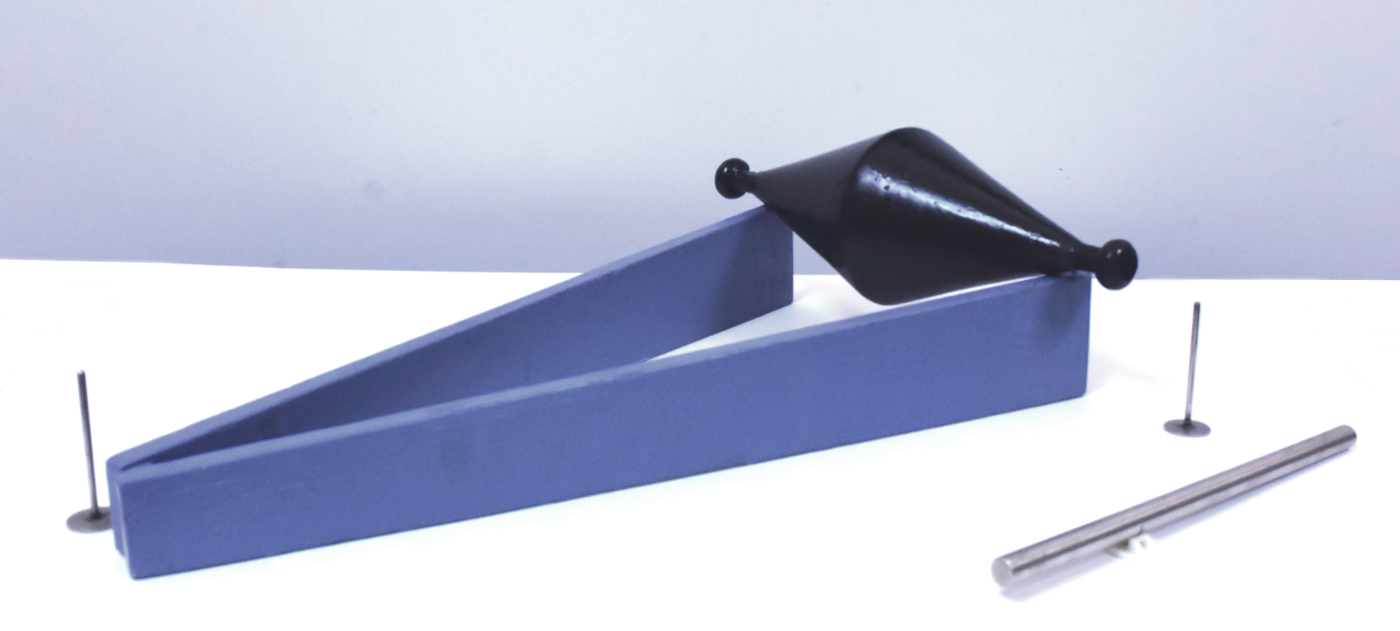
\includegraphics[width=0.9\linewidth]{center-3.png}
		\caption{Демонстрация возможности движения тела в «гору» при опускании его центра масс}
		\label{center-3}
	\end{figure}
	
	\subsection*{\underline{Оборудование:}}
	
	\begin{enumerate} 
		\item Две соединенные между собой рейки переменной ширины
		\item Цилиндрический стержень 
		\item Двойной конус
		\item Метки-указатели
	\end{enumerate}

	\newpage
	\subsection*{\underline{Основные определения:}}
	
	Известно, что центр масс любой механической системы движется точно так же, как и материальная точка, в которой сосредоточена
	Масса всей системы и к которой приложены все внешние силы, действующие на систему.
	
	Потенциальная энергия — часть общей механической энергии системы, зависящая от взаимного расположения частиц, составляющих эту систему, и от их положений во внешнем силовом поле (например, гравитационном).
	Численно такая энергия для системы в данном ее положении равна работе, которую произведут действующие на систему силы при перемещении системы из этого положения в то, где потенциальная энергия минимальна (условно принимается равной нулю).
	
	В случаях сил тяжести и упругости внутренние силы системы стремятся привести тела на нулевой 
	уровень. 
	При приближении тел к нулевому уровню потенциальная энергия системы уменьшается.
	Нулевому уровню действительно соответствует наименьшая потенциальная энергия си	стемы.
	Это означает, что при всех других положениях тел потенциальная энергия системы положительна.

	\subsection*{\underline{Краткое описание:}}
		
		Двойной конус представляет собой тело в виде пары конусов, склеенных друг с другом несимметричным образом.
		Масса внутри такого объекта распределена таким образом, чтобы центр масс двойного конуса не попадал на линию, проходящую через вершины обоих конусов. 
		
		В ходе демонстрации в первую очередь следует показать направление уклона, скатив стержень с «горы».
		Затем необходимо установить в нижней части направляющих двойной конус и обратить внимание на его подъем в «гору».
		
		При помощи пары указателей-меток продемонстрировать, что при подъеме тела в «гору» центр масс конусов опускается.

	\newpage	
		\subsection*{\underline{Теория:}}

	\textit{Опыт 1}. Для начала рассмотрим тело правильной цилиндрической формы  — стержень, лежащий на наклонной плоскости.
	
	На покоящееся тело действует три силы: сила тяжести \textit{m}\textbf{g}, сила реакции опоры \textbf{N} (перпендикулярная наклонной плоскости) и сила трения качения $ \textbf{F}_{\text{тр}} $.
	
	Под действием силы тяжести тело начинает скатываться с наклонной плоскости.
	При этом центр тяжести опускается.
	
	\textit{Опыт 2}. При скатывании двойного конуса, схема принципиально изменяется.
	На схеме (рис.\ref{center-4}) внешняя окружность представляет собой линию соприкосновения двух конусов, из которых изготовлено тело.
	Диаметр этой окружности все время остается неизменным.
			\begin{figure}[H] 	
		\centering 	
		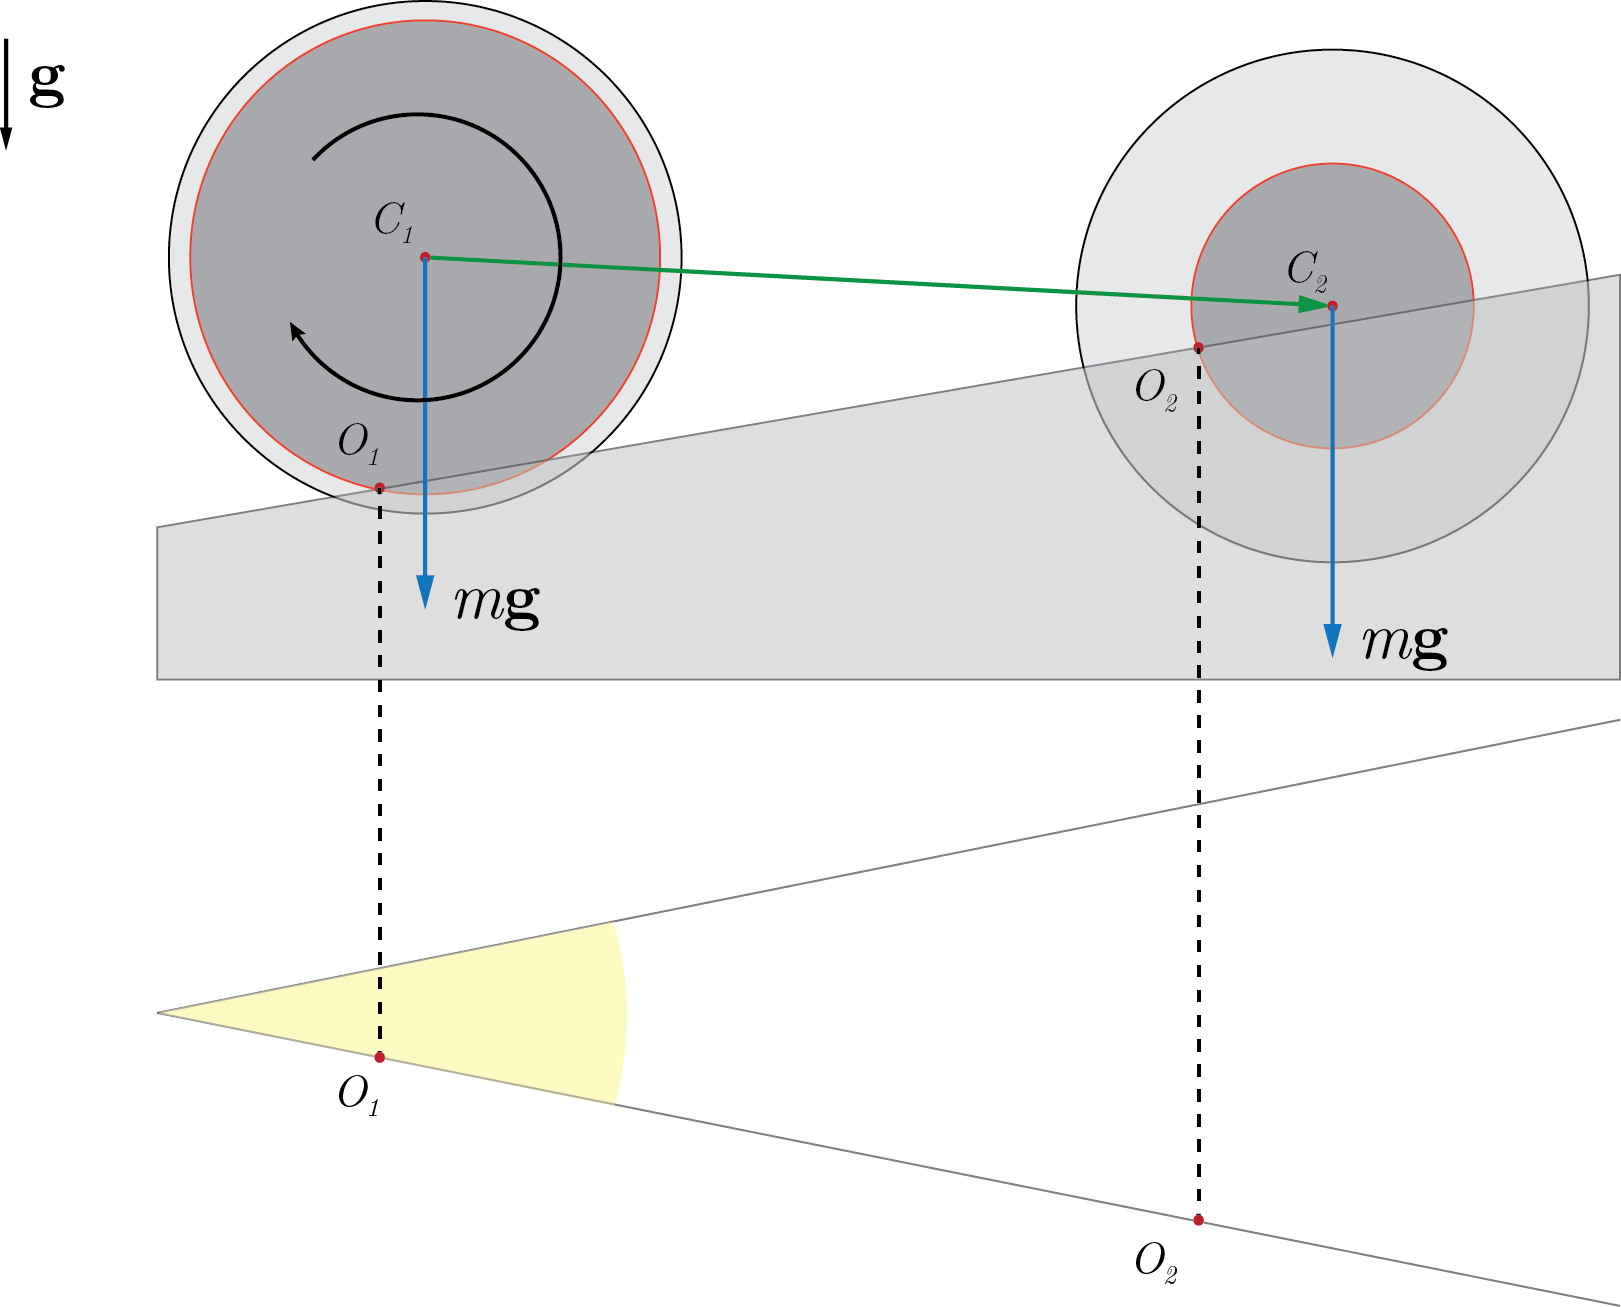
\includegraphics[width=0.75\linewidth]{center-4.png}
		\caption{Демонстрация способа определения центра масс, основанного на свойствах сухого трения}
		\label{center-4}
	\end{figure}

	Внутренняя окружность — это окружность проведенная через точку касания каждого из конусов с наклонной плоскостью.
	 При большом угле между наклонными плоскостями, точки касания располагаются слева от вертикали проходящей через центр тяжести двойного конуса. Поэтому сила тяжести действует на двойной конус таким образом, что приводит к вращению конуса по часовой стрелке. 
	 При этом в опыте наблюдается «подъем» тела по наклонной плоскости.
	 Этот «подъем» объясняется тем, что за счет такого движения центр тяжести конуса в верхнем положении $ C_{2} $ оказывается ниже по сравнению с положением $ C_{1} $.

	Опускание центра тяжести достигается в результате того, что, перемещаясь вверх, конус начинает опираться на свою более узкую часть и благодаря этому центр тяжести конструкции опускается быстрее, чем поднимаются концы.
	Таким образом, опыт показывает, что двойной конус стремиться занять такое положение, в котором его потенциальная энергия оказывается минимальной.
	
\end{document}